\renewcommand{\familydefault}{\sfdefault}

\documentclass{article}
\usepackage{geometry} % Für Layout
\usepackage{geometry}
 \geometry{
 a4paper,
 left=35mm,
 right=50mm,
 top=25mm,
 bottom=25mm,
 footnotesep=20mm,
 }
\usepackage[utf8]{inputenc}
\usepackage{float}
%\usepackage[
%backend=biber,
%style=alphabetic,
%]{biblatex}

%\addbibresource{references.bib} %Imports bibliography file

\usepackage[T1]{fontenc}
\usepackage{hyperref}
\usepackage[ngerman]{babel}
\usepackage{csquotes} % Für Anführungszeichen
\usepackage{hyphenat}
\usepackage{siunitx} % Für SI Symbole
\usepackage{caption}
\usepackage{lipsum} % für Linespacing
\usepackage{setspace} % für Linespacing
\usepackage{footmisc} % für multiple referenced Footnotes
\usepackage{graphicx}
\usepackage{tabularx} % für schöner umgebrochene Tabellen
\usepackage{listings} % um Codezeilen anzuzeigen
\usepackage{color}
\usepackage{float}

\restylefloat{table}

\definecolor{code-background}{RGB}{248,249,250}
\lstset{
    basicstyle=\small\color{black},
    keywordstyle=\color{black}\bfseries,      
    backgroundcolor=\color{code-background}, 
    frame=single, % adds a frame around the code
    captionpos=b, % sets the caption-position to bottom
    breaklines=true, % sets automatic line breaking
}


\graphicspath{ {./images/} }

\hyphenation{Mathe-matik wieder-gewinnen} % Für korrekte Silbentrennung

\title{LoRaWAN Projekt: Sensortree}
\author{Jakob Weirich (\textit{797740}), Michel Schwarz (\textit{843324}) \\und Robert Deppe (\textit{649819})}


\onehalfspacing 

\begin{document}
\setlength{\parindent}{0cm} % Keinen Einzug
\pagenumbering{gobble}  % Keine Seitenzahlen
\onehalfspacing
\maketitle
\newpage

\tableofcontents
\newpage

\subsection*{Aufgabenstellung}
Ziel des Projektes ist die Konzeption und Realisierung einer IoT-Infrastruktur, die es ermöglicht verschiedene Umweltparameter auf dem Campus der Hochschule Düsseldorf zu messen.
Dazu gehören der Kohlenstoffmonoxidgehalt in der Tiefgarage, Temperatur, Luftfeuchtigkeit oder UV-Index.
Die Anbindung der Messstationen an den Server soll über einen WAN Router, ein sogenanntes \textit{LoRaWAN-Gateway} erfolgen.
Spezielle Mikrocontroller (\textit{The Things Uno}) mit eingebautem LoRaWAN-Modul werden dabei als Übermittler der Messdaten an das Gateway verwendet. Die erfassten Daten sollen auf einem Server der Hochschule gespeichert werden und über eine Benutzeroberfläche zugänglich gemacht werden.

% \vfill{}

% \begin{abstract}
%     Abstract
% \end{abstract}

% \vfill{}

\newpage

\setcounter{page}{1}
\pagenumbering{arabic}

\section{Einleitung}

In den letzten Jahren haben IoT (Internet of Things) Anwendungen in allen Bereich unseres Lebens Einzug gefunden. 
Dazu zählen Bereiche im Gesundheitswesen, im Energiesektor oder in einer Smart City.
Die Möglichkeiten die durch IoT Anwendungen entstehen sind vielfältig.
Dadurch dass Hardware zunehmend günstiger und die Implementierung immer leichter wird, können Projekte realisiert werden, die unsere Umwelt analysieren oder beeinflussen.
Sensornetzwerke sind in der Lage kleinste Veränderungen in unserer Umgebung zu registrieren und aufzuzeichnen. Sie bieten damit die Grundlage für umfangreiche Analysen.
Innerhalb dieses Projektes soll eine IoT-Anwendung entstehen, die diese Vorteile nutzt und eine Langzeitaufzeichnung von Umweltdaten an der Hochschule Düsseldorf erstellt.
Die Anwendung soll in einer interaktiven Webseite die aktuelle Temperatur, Luftfeuchtigkeit und den Kohlenstoffmonoxidgehalt darstellen.\\
\\
Die Webseite selbst, sollte so aufgebaut sein, dass in einem responsiven Design die gespeicherten Messwerte leicht ermittelt werden können.
Ein Framework wurde integriert um die Daten in einer anschaulichen Grafik zu visualisieren.
Die gesamte Software-Struktur sollte auf einem Server der Hochschule Düsseldorf untergebracht werden. Dazu zählen die Datenbank, das Front-End und der Back-End-Server.
Die Hardware für dieses Projekt wurde zusammengestellt und in einer kleinen elektrischen Schaltung installiert.
Um die Daten auszulesen wurde der Mikrocontroller Arduino gewählt.
Dazu mussten passende Sensoren ausgewählt werden, die gleichzeitig kompatibel mit diesem Mikrokontroller sind.\\
\\
Für die Kommunikation zwischen dem Server der Hochschule Düsseldorf und der Hardware wurde die Anwendung innerhalb des TTN (The Things Network) betrieben.
TTN verwendet ein Netzwerkprotokoll vom Typ \textit{Long Range Wide Area Network} (LoRaWAN). Dieses ermöglicht das energieeffiziente und weitreichende Senden von Daten innerhalb eines Netzwerkes.
TTN bietet hierfür vorpräparierte Hardware an.
Dazu zählen ein Gateway welches die Verbindung in das Internet ermöglicht und ein Arduino Uno welcher bereits über ein LoRaWAN Modul verfügt.

% In den letzten Jahren ist Hardware für spezielle Anwendungsfälle durch sinkende Preise und unmittelbarere Verkaufsketten zugänglicher für Amateur- und semiprofessionelle Anwendungsfälle geworden. % TODO: CITATION NEEDED
% % TODO: Beschreibung Entstehung LoraWAN
% Diese Entwicklung förderte eine breite Popularisierung von Smart-Home Systemen und verteilten Sensornetzwerken, sowohl kommerziell als auch in einem privatem Umfeld. % TODO: CITATION NEEDED


\newpage

\section{Hardware der Sensorstation}
% Notizen für Arduino - Hardware
\subsection{CO Sensor}
Der verwendete Gassensor ist ein Figaro Gas-Sensor mit der Bezeichnung "TGS-2620" \cite{figaro-gas-sensor}.
Dieser kann für die Gase Isobutan, Methangas, Wasserstoff, Kohlenmonoxid, Methylmercaptan und Hydrogens verwendet werden.
Der Sensor verfügt über einen Heizstab der an eine Spannungsversorgung von 5 VDC angeschlossen werden muss.
Der Sensor benötigt für einen optimalen Betrieb einen Widerstand RL.
Über diesen Widerstand wird die Sensitivität des Sensors gesteuert.
Dadurch kann definiert werden welches Gas ermittelt werden soll.
Für unseren Fall wurde für RL \SI{10}{\kilo\ohm} gewählt.\\

\begin{figure}[h]
 \centering
 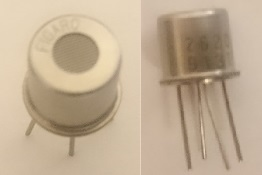
\includegraphics[height=3cm]{images/CO_Sensor.JPG}
 \caption{CO Sensor}
 \label{fig:co_sensor}
\end{figure}

Der Sensor verfügt über vier Anschlüsse.
\begin{center}
\begin{tabular}{|c|p{0.9\textwidth}|}
    \hline
    1 & Spannungsversorgung für den Heizstab \\ \hline
    2 & Negative Sensorelektrode \\ \hline
    3 & Positive Sensorelektrode\\ \hline
    4 & Spannungsversorgung für den Heizstab\\ \hline
\end{tabular}
\end{center}


\subsection{Feuchtigkeits - und Temperatursensor}
Der Kombinationssensor von JOY-IT mit der Kennung "SEN-KY015" misst die Feuchtigkeit und die Temperatur \cite{joy-it-sensor}.
Der Messbereich für die Temperatur liegt bei 0 - \SI{50}{\degreeCelsius} und bei der Luftfeuchtigkeit bei 20 - 90\%.
Um den Sensor in Betrieb nehmen zu können, wird eine Betriebsspannung von 5 VDC benötigt.
Auf dem Sensor ist ein Chipsatz (DHT11) angebracht, der dafür sorgt, dass die Messwerte als digitales kodiertes Signal an den Arduino weitergegeben werden.
Für diesen Chipsatz wird vom Hersteller eine Bibliothek bereitgestellt um diesen Sensor mit einem Arduino zu betreiben.
Diese Bibliothek wurde in das Programm für die Campus-Klima-App integriert um die Daten auszulesen.\\

\begin{figure}[h]
 \centering
 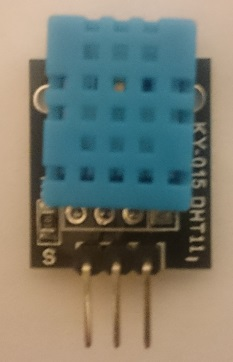
\includegraphics[height=4cm]{images/Temp_Sensor.JPG}
 \caption{Feuchtigkeits - und Temperatursensor}
 \label{fig:temp_sensor}
\end{figure}

Der Sensor hat drei Anschlüsse. 
\begin{center}
\begin{tabular}{|c|p{0.9\textwidth}|}
    \hline
    1 & Digitales Signal \\ \hline
    2 & Spannungsversorgung 5 VDC \\ \hline
    3 & GND \\ \hline
\end{tabular}
\end{center}
\newpage
\subsection{The Things Uno}
Der \textit{The Things Uno} ist ein Arduino Mikrocontroller, der auf dem Arduino Leonardo basiert.
Dieser ist mit einem LoRaWAN-Modul ausgestattet, das die Kommunikation mit dem \textit{The Things Network} (TTN) ermöglicht. 
Jedes einzelne Gerät muss vor dem eigentlichen Betrieb auf der TTN-Webseite registriert sein.
Dadurch kann eine Verbindung zum TTN hergestellt und Daten übertragen werden\cite{TheThingsNetwork-Uno.2020}.\\

Durch das TTN Gateway können die Geräte des TTN miteinander kommunizieren.
Dazu muss das Gateway ebenfalls auf der TTN-Webseite registriert und mit dem Internet verbunden werden.
Zu beachten ist hierbei, dass die richtige Frequenz in den einzelnen Geräten des TTN gewählt wird. 
Für Geräte in Europa ist eine Frequenz von 868 MHz vorgesehen. 
Für Geräte aus den USA ist eine Frequenz von 915 Mhz vorgesehen.
Diese Frequenz muss in der Software für das jeweilige Gerät angegeben werden\cite{TheThingsNetwork-Gateway.2020}.\\


\begin{figure}[h]
 \centering
 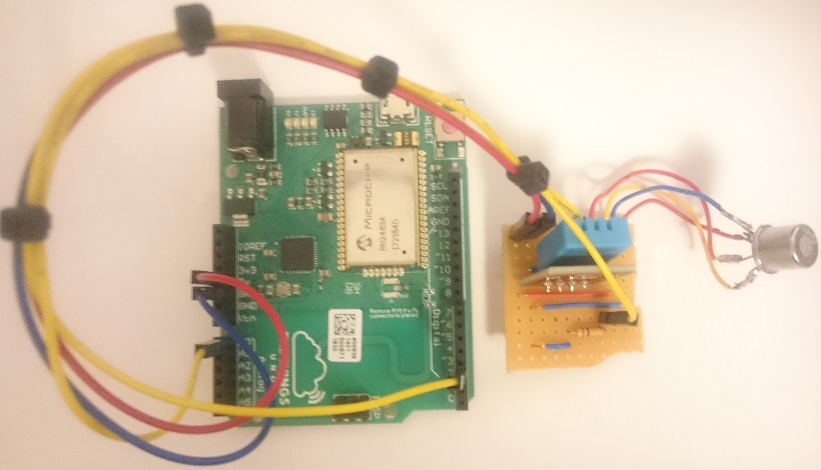
\includegraphics[height=4cm]{images/Arduino_Uno.JPG}
 \caption[Foto der Hardware]{Arduino Uno verbunden mit selbst zusammengelöteter Sensorplatine}
 \label{fig:schaltplan_uno}
\end{figure}

\subsection{Schaltplan}
Für die Hardware der Campus-Klima-App wurde der Schaltplan für den CO Sensor modifiziert, indem der Feuchtigkeits- und Temperatursensor integriert wurde.
Die Schaltung ist in Abbildung ~\ref{fig:schaltplan} zu sehen und wurde auf einer Lochrasterplatine verlötet.

\begin{figure}[h]
 \centering
 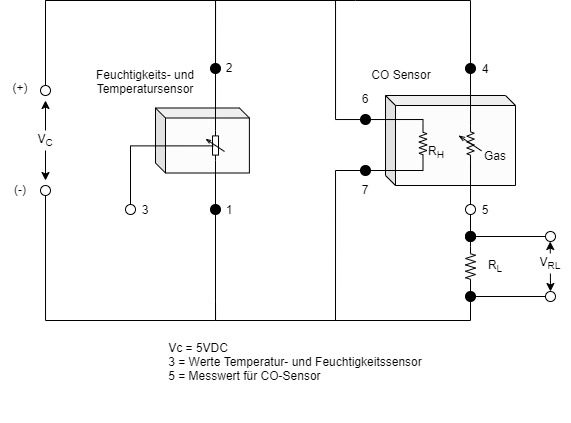
\includegraphics[height=9cm]{images/Schaltplan_Sensoren}
 \caption{Elektrischer Schaltplan für die Sensoren}
 \label{fig:schaltplan}
\end{figure}

\newpage

\section{Software}
Das Zusammenspiel der verschiedenen Software-Komponenten ist so angelegt, dass es einfach erweitert oder einzelne Bestandteile ausgetauscht werden können.
Die Kommunikation der, an das Internet angeschlossenen Komponenten, ist über REST-Aufrufe realisiert, die auf weit verbreiteten HTTP-Anfragemethoden basieren.\\

In Abbildung~\ref{fig:software_structure} wird der Weg eines vom Sensor ermittelten Datums bis zur Darstellung in der Web-App beschrieben.
Zu Beginn wird in regelmäßigen Intervallen der Wert der Sensoren vom Arduino-Mikrocontroller ausgelesen.
Die analogen Werte werden hier digitalisiert und als Messwerte interpretiert, während die digitalen Messwerte bereits interpretiert von der Sensorplatine an den Arduino geschickt werden.
Im nächsten Schritt sendet der Arduino die Werte über LoRaWAN-Funk an einen \textit{The Things Network}-Router in der Umgebung, welcher als Schnittstelle zur Online-Plattform \textit{The Things Network} fungiert.
In diesem ist ein Plugin für unser Projekt aktiviert, welches bei neuen Daten einen Webhook-Request auslöst, welcher an eine hinterlegte URL geht.
In unserem Fall ist dies unser Backend-Server, der den HTTP-Request empfängt und die Daten strukturiert in einer MongoDB hinterlegt.
Wird nun das Front-End auf einem Endgerät aufgerufen, fragt dieses ebenfalls den Back-End Server über einen HTTP-Request an, und erhält die Daten für den angegebenen Zeitraum.
Diese werden nun als Diagramm visualisiert und ausgewertet dargestellt.

\begin{figure}
    \centering
    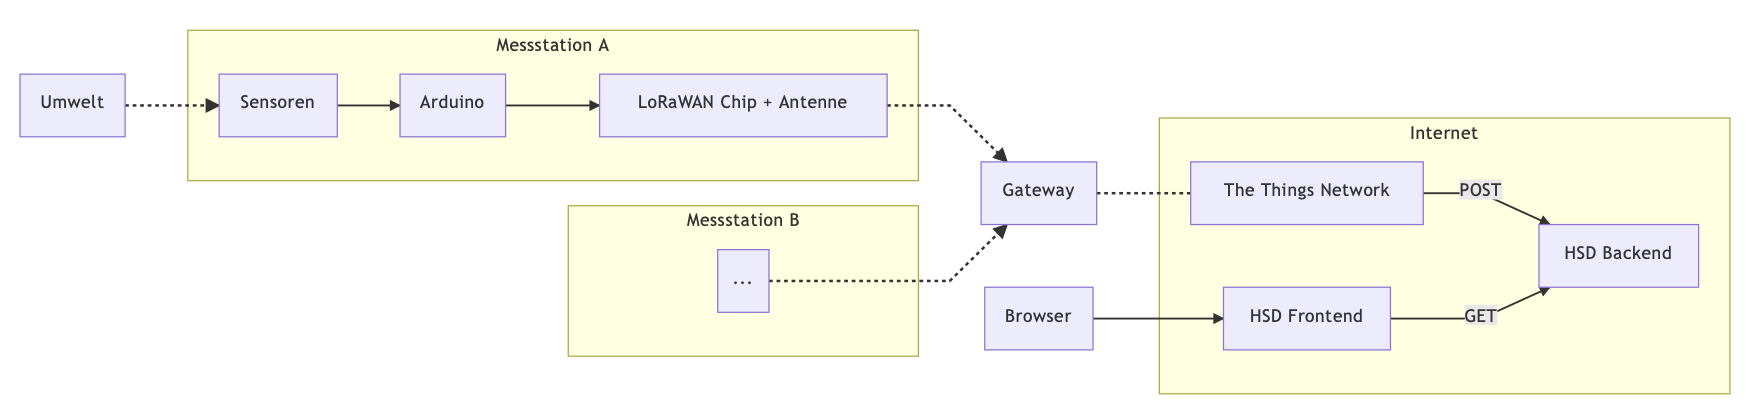
\includegraphics[width=\textwidth]{images/Software_structure}
    \caption{Zusammenspiel der verschiedenen Softwarekomponenten}
    \label{fig:software_structure}
\end{figure}

% TODO: Allgemeiner Aufbau mit Diagramm
% Dabei daran denken, dass DB, Front- und Backend nicht auf einem Server liegen müssen!
% Zusammenspiel mit TTN-Webhook beschreiben

\subsection{Arduino-Software}
Durch TTN wurden bereits Beispielprogramme für den Arduino Uno angeboten.
Die Bibliothek hierfür wurde integriert und das Programm zum Teil modifiziert.
Die Modifizierungen beziehen sich auf die Integration der Sensoren.
Hierbei musste zum Einen die DHT Bibliothek für den Feuchtigkeits - und Temperatursensor importiert werden. 
Für diesen Sensor war ebenfalls ein Beispielprogramm bereits vorhanden. 
Die Messwerte, die dieses Programm ermittelt, sind digital und mussten lediglich in Bytes umgewandelt und an TTN gesendet werden.\\
Für den Code-Abschnitt, der sich mit dem CO Sensor befassen sollte, wurde eine Quelle im Internet gefunden, welche sich mit diesem Problem befasste \cite{seeed-wiki}.
Diese Quelle wurde als Leitfaden für die Ermittlung der Gas Werte genommen.\\
\\
Die Messwerte für den CO Sensor wurden analog eingelesen. Hierfür war eine Umrechnung notwendig, um am Ende Werte in Bytes zu erhalten.
Um korrekte Werte zu erhalten, mussten anfangs Messwerte in der Luft ermittelt werden. Der entscheidende Code-Abschnitt im Programm ist hierfür in Listing~\ref{list:co-sensor-luft} zu sehen.
In der Abbildung ~\ref{fig:gas_sensitivität} ist zu sehen, dass der Wert für Lust ermittelt abgelesen werden kann. Die Abbildung stammt aus der offiziellen Dokumentation des Herstellers \cite{gas-sensor-datenblatt}.

Dieser Wert wurde im Code zur Ermittlung von R0 eingegeben.
Nachdem R0 ermittelt und ausgegeben wurde, konnte dieser der Wert für R0 in Listing~\ref{list:co-sensor-gas} eingefügt werden.
Der Wert sorgt dafür, dass das Programm die Werte für Kohlenstoffmonoxid berechnet.
Hierbei muss festgehalten werden, dass diese Kalibrierung nicht unter Laborbedingungen stattgefunden hat.
Bevor der Sensor in einer realen Umgebung in Betrieb genommen werden kann, sollte diese Kalibrierung wiederholt werden.

\begin{lstlisting}[language=Bash, caption=Messung des CO Sensors für Luftwerte, label=list:co-sensor-luft]
    float RS_air; 
    float R0;  

    R0 = RS_air/21.0; 
 
    Serial.println(R0);
\end{lstlisting}

\begin{figure}[h]
 \centering
 \includegraphics[height=8cm]{images/gas_sensitivitäts_diagramm_(RsRo).JPG}
 \caption{Gas Sensitivität für RS/R0}
 \label{fig:gas_sensitivität}
\end{figure}

\begin{lstlisting}[language=Bash, caption=Messung des CO Sensors, label=list:co-sensor-gas]
    float sensor_volt;
    float RS_gas; 
    float ratio; 
    int sensorValue = analogRead(A0);

    RS_gas = (5.0-sensor_volt)/sensor_volt; 

    ratio = RS_gas/R0;
\end{lstlisting}
% Fehler im Code: Die Initialisierung im Code war nicht korrekt. 
% Es fehlte das sensorValue auf den Wert 0 in der Loop() %Funktion zurück gesetzt wird. 
% Dadurch wurde der sensorValue endlos aufsummiert und es wurden falsche Werte ausgegeben.

% Um die korrekten Werte für unseren Sensor bestimmen zu können haben wir aus der Grafik Fig. 4 - Sensitivity to various gases (Rs/Ro) den Wert für das Verhältnis von Rs/R0.

% R0 wird mit dem folgenden Programmteil ausgerechnet.
% R0 = RS_air/21.0;


\subsection{Back-End}
Der Zugriff auf die Datenbank erfolgt über eine REST-API, welche in Form einer separaten Anwendung läuft.
Diese entkoppelt die verwendete Datenbank vom Front-End, was eine Skalierung oder Modifizierung von Teilen des Systems vereinfacht.
Im Falle unserer Umsetzung erfolgt dieses auf dem selben Server, kann jedoch auch auf mehrere Systeme verteilt werden um unterschiedlichen Anforderungen gerecht zu werden.

Die Daten werden über diese API übermittelt. Das TTN sendet in regelmäßigen Abständen einen Datensatz an die URL des Back-Ends. 
Dieses stellt hierfür HTTP Request Methoden zur Verfügung. Innerhalb des Back-Ends werden die Daten dann in ein Schema umgewandelt.
Dies soll gewährleisten, dass nur die notwendigen Daten in einer übersichtlichen Form in der Datenbank abgelegt werden.
Gleichzeitig kann das Front-End ebenfalls über diese Methoden die Daten aus der Datenbank auslesen. Somit ist das Front-End unabhängig vom jeweilig verwendeten Datenbank Management System.
REST-Routen der API:
\begin{itemize}
    \item \textbf{POST} \texttt{/datapoints} --- Fügt einen Datenpunkt zur Datenbank hinzu. Hierbei wird das JSON-Objekt, welches vom TTN-Webhook kommt in das Datenbankmodell übersetzt.
    \item \textbf{GET} \texttt{/datapoints} --- Gibt alle Datenpunkte von allen verfügbaren Sensorstationen zurück
    \item \textbf{GET} \texttt{/datapoints/\{device\_id\}}  --- Gibt alle Datenpunkte des angegebenen Sensorstationen zurück.
\end{itemize}
Bei den beiden \textbf{GET}-Requests kann optional auch ein \texttt{from} und \texttt{to} HTTP-Header in die Anfrage gegeben werden, welcher als Datum geparsed wird und den angefragten Datensatz auf den gewünschten Zeitraum reduziert.
Außerdem ist es möglich den boolischen Header \texttt{include\_all\_fields} mitzugeben, wodurch nicht nur \textit{Datensatz-ID}, \textit{Sensorstation}, \textit{Lichtlevel}, \textit{Temperatur} und \textit{Zeitpunkt}, sondern auch \textit{Batteriestatus}, \textit{Event-Art} und \textit{Rohdaten}, sofern vorhanden, zurückgegeben werden.

\subsection{Front-End}
Die Basis für das Front-End bietet die JavaScript Bibliothek \href{https://reactjs.org}{React.js} - oft einfach nur React genannt, mit dessen Hilfe die Erstellung von dynamischen Benutzeroberflächen vereinfacht wird.
Entwickelt wurde das Open-Source Webframework ursprünglich von Facebook, weshalb es erstmalig für den Facebook Newsfeed sowie später für Instagram verwendet wurde.
Seitdem hat es stark an Popularität gewonnen und kommt heute auf zahlreichen Webseiten wie \textit{Airbnb}, \textit{Dropbox}, \textit{Microsoft}, \textit{Yahoo} oder \textit{Netflix} zum Einsatz.\\

Ein Vorteil von React gegenüber klassischen HTML basierten Anwendungen besteht darin, dass eine Webseite aus einer Vielzahl von funktionalen Untereinheiten, sogenannte Komponenten zusammengesetzt wird, welche von React später als HTML-Markup gerendert werden.
In einer Komponente gehört die Logik bzw. die Methoden sowie das Markup in Form von JSX zusammen.
Damit wird uns erleichtert einen besseren Überblick über den Code zu behalten und ermöglicht eine funktionierende Komponente in Zukunft erneut zu verwenden. Beispiele von Komponenten in diesem Projekt sind die Anzeige zur Darstellung der Punkte mittels SVG, das Menü, die Auswahl des Zeitraums oder die Buttons über der Grafik.\\

DOM Manipulationen sind oft rechenintensiv und reduzieren damit die Reaktionsgeschwindigkeit der Seite.
Deshalb pflegt React einen virtuellen DOM, also eine interne Repräsentation des DOMs, an dem vorerst die Manipulationen geschehen.
Die Differenz zwischen dem Zustand des virtuellen DOMs und dem des DOMs bestimmt letztendlich, welche Veränderungen am realen DOM vorgenommen werden.
Somit wird vermieden, dass bei jeder Veränderung die gesamte Grafik erneut berechnet werden muss.\\


Um die Vektorgrafik, in Form von SVG, zu erzeugen, wird auf eine weitere JavaScript-Bibliothek namens D3.js zurückgegriffen.
Der Ansatz von D3 ist, dass der DOM basierend auf einem vorhandenen Datensatz verändert wird. Das Kernkonzept, des sogenannten "`Data-Bindings"', weist in unserem Fall jedem visuellen Punkt-Element genau ein Daten-Element zu.
Verändert sich der Datensatz, werden die Attribute (Lage abhängig von der X- und Y-Skala sowie Größe) der vorhandenen Punkte aktualisiert, oder, sofern sich die Anzahl der Daten verändert hat, neue Punkte erzeugt bzw. entfernt.
Weitere bereitgestellte Funktionen von D3 erleichtern die Berechnungen für Skalen sowie das Zeichnen der Achsen.

\vspace{0.5cm}

\begin{figure}[H]
    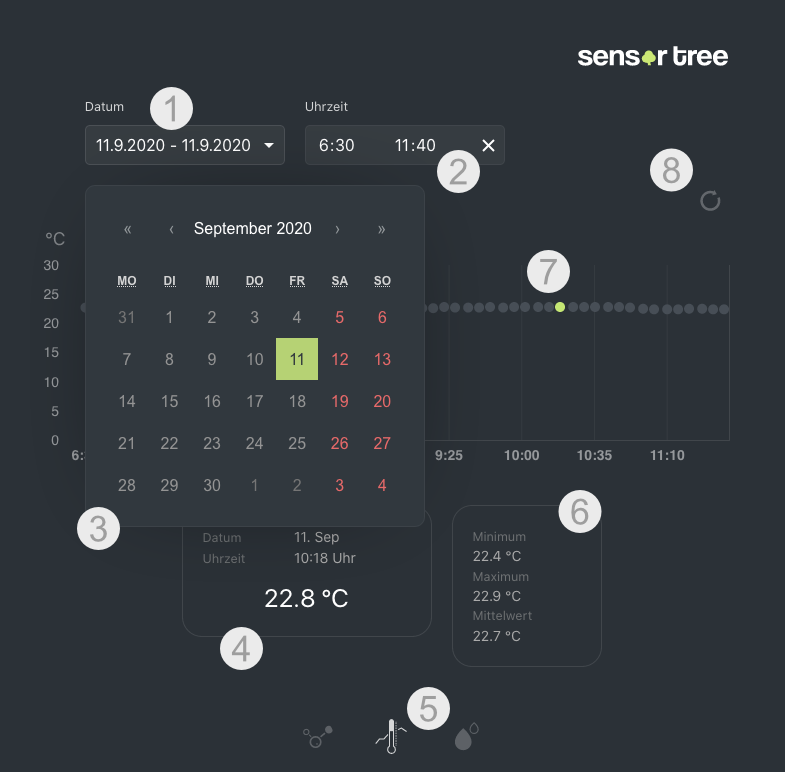
\includegraphics[width=\textwidth]{ui-with-dots}
    \centering
    \caption{Benutzeroberfläche mit Kalender}
    \label{fig:Benutzeroberfläche mit Kalender}
\end{figure}

\begin{table}[H]
\begin{tabular}{|c|p{0.9\textwidth}|}
    \hline
    1 & Button zum Anzeigen und Schließen des Kalenders; zeigt den ausgewählten Zeitraum als Datum an \\ \hline
    2 & Eingabefelder für den Zeitraum als Uhrzeit; Kreuz löscht die Eingabe und setzt den Standardwert von 0:00 - 23:59 Uhr\\ \hline
    3 & Kalender zur Auswahl des Start- und Enddatums; zur Auswahl eines Tages werden für Anfang und Ende der selbe Tag ausgewählt\\ \hline
    4 & Anzeige der Daten zum ausgewählten Punkt in der Vektorgrafik \\ \hline
    5 & Menü zum Wechseln zwischen verschiedenen Umweltparametern: Kohlenstoffdioxid (links), Temperatur (Mitte) und Luftfeuchtigkeit (rechts)\\ \hline
    6 & Anzeige von Minimum, Maximum sowie Mittelwert der Daten im ausgewählten Zeitraum \\ \hline
    7 & Ausgewählter Datenpunkt; Auswahl erfolgt über Klicken/Tippen auf den Punkt\\ \hline
    8 & Button zum Aktualisieren der Daten; \textit{Hinweis: Daten werden automatisch alle 5 Minuten aktualisiert} \\ \hline
\end{tabular}
\end{table}

\subsection{Datenbank}
Um die gemessenen Daten zu sammeln und im Front-End visualisieren zu können, musste ein DBMS integriert werden. 
Dazu wurde die dokumentenorientierte Datenbank MongoDB gewählt. Diese ist sehr flexibel und strukturlos verwendbar. 
Die darin enthaltenen Dokumente werden in einer JSON-Struktur abgelegt, wobei hier jedes Dokument einen anderen Aufbau besitzen kann. 
Die Struktur die unsere Dokumente in der Datenbank besitzen werden lediglich durch die das Schema, welches im Back-End definiert wurde, vorgegeben\cite[3-5]{Hows.2015}. \\

Um die Daten besser beibehalten zu können wurde auf dem Hochschulserver ein Replica-Set initialisiert. 
Das heißt, dass nicht nur eine einzelne Datenbank die Daten speichert, sondern das ein Cluster aus drei Datenbanken betrieben wird. 
Die beiden Replikanten, auch Secondarys genannt, erhalten von der primären Datenbank ein Oplog (operations log). 
Dieses beinhaltet alle Änderungen die in der Primären Datenbank durchgeführt wurden. 
Die beiden sekundären Datenbanken führen alle Aufzeichnungen aus dem Oplog durch und besitzen somit den gleichen Datenbestand wie die primäre Datenbank\cite[289-291]{Hows.2015}.\\

Dieses Cluster wurde initialisiert, um das System auf eine mögliche Verteilung vorzubereiten. 
Somit kann zu einem späteren Zeitpunkt eine Datenbank auf einem anderen Server betrieben werden und muss lediglich in das bisherige System integriert werden. 
Der nachfolgende Code zeigt, wie in einem Linux-System ein Keyfile erstellt wird um die Authentifizierung zwischen den Datenbanken zu gewährleisten.\\
\begin{lstlisting}[language=Bash, caption=Erstellen eines Keyfiles]
openssl rand -base64 756 > <path-to-keyfile>
chmod 400 <path-to-keyfile>
\end{lstlisting}

Damit ein Cluster erfolgreich untereinander kommuniziert, muss nach dem Start der Docker-Container eine initiate-Funktion durchgeführt werden. 
Diese wurde bereits in das Docker-Image integriert.
Dennoch benötigt die MongoDB eine rsconfig() Funktion um die Verbindung erneut einzuleiten \cite[304-306]{giamas2019mastering}.
Diese ist in Listing~\ref{list:rsconf} zu sehen.

\begin{lstlisting}[ caption=MongoDB initiate() Funktion, label=list:rsconf]
rsconf = rs.conf();
rsconf.members = [
    { _id : 0, host : "cka-mongodb1:27017" },
    { _id : 1, host : "cka-mongodb2:27017" },
    { _id : 2, host : "cka-mongodb3:27017" }
];
rs.reconfig(rsconf, {force: true});
rs.slaveOk();
\end{lstlisting}

Auch mussten alle Benutzer neu angelegt werden. Darunter fällt der Administrator und ein Benutzer über den die Campus-Klima-App den Login vornehmen kann. 
Beide Benutzer wurden ebenfalls erstellt und sind innerhalb des Docker-Images integriert.  \\
\newpage
Die Daten für die Campus-Klima-App werden in der Kollektion "`datapoint"' abgelegt.
Dieser Name der Kollektion wurde so auch im Backend definiert. 
Um eine neue Kollektion festzulegen oder den Namen zu ändern, muss somit auch der Name im Backend geändert werden.
Die Kollektion in der MongoDB hat keine vordefinierte Struktur.
Die Struktur der Dokumente wird allein durch den Request des Back-Ends definiert.
\begin{lstlisting}[caption=Eine Dokument für mit Sensordaten, label=dataset]
{
        "_id" : ObjectId("5f5b75bdcb14433649394736"),
        "device_id" : "arduino",
        "co" : 156,
        "humidity" : 56,
        "raw" : "CKwV4ACc",
        "temperature" : 22.2,
        "time" : ISODate("2020-09-11T13:03:56.951Z"),
        "__v" : 0
}
\end{lstlisting}
\subsection{Docker}
Docker ist ein Containersystem, welches eine Virtualisierung anbietet, die im Vergleich zu virtuellen Maschinen deutlich weniger Ressourcen benötigt. 
Dadurch können einzelne Container erstellt werden, wobei jeder Container ein unterschiedliches Image beherbergt.
Diese Images sind im Falle der Campus-Klima-App das Node.js Back-End, das React Front-End und drei Instanzen eines MongoDB Clusters.\\

Der Container selbst wird über den Docker-Daemon adressiert. Das bedeutet, dass Requests, die an die Host-Maschine gesendet werden, an die Container weitergeleitet werden.
Damit der richtige Container adressiert wird, muss vorher noch ein Port definiert werden.
Dabei wird zwischen dem Port innerhalb und außerhalb des Containers unterschieden. 
Ein äußerer Port kann nur einmalig vergeben werden. 
Zum Beispiel werden alle Anfragen auf localhost:80 an den Container, in dem der Node.js Back-End Server implementiert ist, gesendet. Der Node.js Server im Container selbst, hört aber auf den Port 3000 \cite[12-13]{Vohra.2016}.\\
%%
%% Quelle: Vohra.2016 Seite 12-13
%%

\begin{figure}[h]
 \centering
 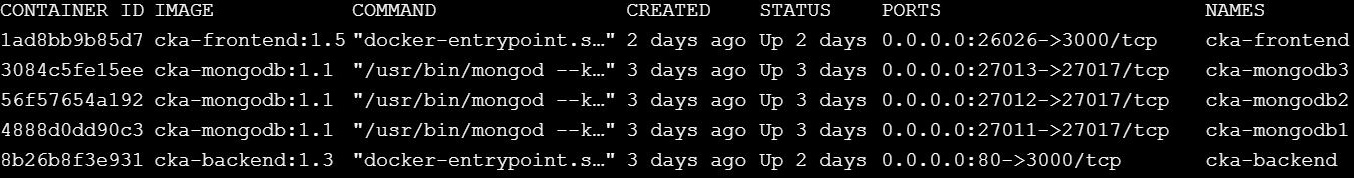
\includegraphics[height=1.7cm]{images/cka-container-docker-ps}
 \caption{Docker Container auf dem Server}
 \label{fig:Docker Container auf dem Server}
\end{figure}

In Abbildung~\ref{fig:Docker Container auf dem Server} ist zu sehen, dass auf dem Server der Hochschule Düsseldorf fünf Container gestartet wurden. Das jeweilige Image zum Starten eines Servers wurde eigens definiert und auf dem Server abgelegt.
\newpage
\section{Fazit}
Die Campus-Klima-App zeigt die Umweltmesswerte in einer überschaubaren und informativen Grafik an. Das Front-End wurde so entwickelt, dass alle notwendigen Informationen für den Betrachter leicht zu erkennen sind.
Hierbei muss aber beachtet werden, dass das Front-End noch erweitert werden kann.
Beispielsweise könnte noch ein Sensor für den UV-Index integriert werden oder der Batteriestatus der einzelnen Messstationen.
Somit kann festgehalten werden, dass die Campus-Klima-App in seiner momentanen Form noch modifiziert werden kann. 
Dieses Projekt enthält eine Server-Struktur, die es zukünftigen Entwicklern ermöglicht, leicht Änderungen vorzunehmen.
So kann die App, ohne viel Aufwand und ohne die Struktur neu aufsetzen zu müssen, an die jeweiligen Bedürfnisse der Hochschule Düsseldorf angepasst werden.
Die Messergebnisse für den CO Sensor sind bislang noch nicht unter Laborbedingungen erfasst worden.
Um die Messwerte zu validieren, sollten die Werte des CO-Sensors überprüft werden.
Dies kann in einer kontrollierten Umgebung geschehen, indem Vergleichswerte herbeigezogen und Umwelteinflüsse, die zu einer Verfälschung der Messwerte führen könnten, reduziert werden.

\newpage

\listoffigures
\newpage

\newpage

\pagenumbering{gobble}  % Keine Seitenzahlen
\section*{Eidesstattliche Erklärung}
Hiermit erklären wir, Jakob Weirich, Michel Schwarz und Robert Deppe dass wir die vorliegende Arbeit selbstständig und ohne unerlaubte Hilfe angefertigt, andere als die angegebenen Quellen und Hilfsmittel nicht benutzt und die den benutzten Quellen wörtlich oder inhaltlich entnommenen Stellen als solche kenntlich gemacht haben.


\newpage
\bibliographystyle{ieeetr}
\bibliography{references}{}
\end{document}
